\chapter{Evaporation from Water Surfaces} \label{chap:evap}
\renewcommand{\tabdir}{chapters/part_processes/evaporation/tab}
\renewcommand{\figdir}{chapters/part_processes/evaporation/fig}

\section{Introduction} \label{sec:evap_intro}

This chapter introduces evaporation models. The approach(es) can be used to estimate the water losses associated with evaporation from lake, reservoir, and river surfaces.

%%%%%%%%%%%%%%%%%%%%%%%%%%%%%%%%%%%%%%%%%%%%%%%%%%%%%%%%%%%%%%%%%%%%%%%%%%%%%%%%
%%%%%%%%%%%%%%%%%%%%%%%%%%%%%%%%%%%%%%%%%%%%%%%%%%%%%%%%%%%%%%%%%%%%%%%%%%%%%%%%
%%%%%%%%%%%%%%%%%%%%%%%%%%%%%%%%%%%%%%%%%%%%%%%%%%%%%%%%%%%%%%%%%%%%%%%%%%%%%%%%

\section{Makkink model} \label{sec:evap_makkink}

The Makkink model is a simple empirical equation to estimate evaporation using a minimum set of input data, namely short wave radiation and air temperature. In has been derived for the Netherlands. Using convenient units, the basic equation is (\eqnref{eqn:evap_makkink_main})

\begin{equation} \label{eqn:evap_makkink_main}
  e = c \cdot \frac{s}{s + \gamma} \cdot \frac{\radShortwaveIn}{1000 \cdot \evapHeatWater \cdot \densityWater} + b
\end{equation}

with

\begin{tabular}{lp{0.8\columnwidth}}
  $e$ & Makkink reference evaporation (m/s) \\
  $s$ & Slope of the curve of saturation water vapor pressure (kPa / K) \\
  $\gamma$ & Psychrometric constant (kPa / K) \\
  $\radShortwaveIn$ & Incoming short-wave radiation (W/\sqm{}) \\
  $\evapHeatWater$ & Latent heat of water evaporation (kJ/kg). \\
  $\densityWater$ & Density of water ($\approx$ 1000 kg/\cbm{}). \\
  $c$ & Empirical factor (--). \\
  $b$ & Empirical correction term (m/s). \\
\end{tabular}

\medskip
One should realize that only the incoming short-wave radiation is used in \eqnref{eqn:evap_makkink_main}, thus other terms of the energy balance, such as reflection (albedo), long wave emissions, and heat storage are all neglected.

For the dimensionless term $s/(s + \gamma)$ \citet{Yao2009} present a convenient approximation based on the air temperature \airtemp{} in units of \celsius{}  (\eqnref{eqn:evap_makkink_dimlessFraction}). The error from using this approximation is < 4~\% for temperatures between 4 and 30~\celsius{} and about 7~\% at 0~\celsius{} when compared to the equations for separate estimation of $s$ and $\gamma$ given in \citet{Hiemstra2011}.

\begin{equation} \label{eqn:evap_makkink_dimlessFraction}
  \frac{s}{s + \gamma} \approx 0.439 + 0.01124 \cdot \airtemp
\end{equation}

The latent heat of water evaporation \evapHeatWater{} (kJ/kg) can be estimated from the water temperature $T$ (\celsius) using \eqnref{eqn:evap_makkink_evapHeatWater} \citep{Hiemstra2011}. Since water temperature data are usually unavailable, the air temperature \airtemp{} must be used as a substitute for $T$.

\begin{equation} \label{eqn:evap_makkink_evapHeatWater}
  \evapHeatWater = 2501 - 2.375 \cdot T
\end{equation}

For the two empirical parameters, \citet{Winter1995} report values of $c= 0.61$ and $b=-0.012/100/86400$ (unit of $b$ converted from cm/d to m/s). \citet{Hiemstra2011} suggest $c = 0.65$ and $b = 0$ but their report does not explicitly focus on evaporation from water surfaces.

\tabref{tab:evap_makkink_example} provides some results of the application of \eqnref{eqn:evap_makkink_main} for selected temperatures and short-wave radiation inputs.

\begin{table}
  \caption[Makkink evaporation for different values of temperature and daily-average short-wave radiation.]{Makkink evaporation (mm/day) for different values of temperature (\celsius{}) and daily-average short-wave radiation (W/\sqm). The empirical parameters were set to $c=0.61$ and $b=-0.012/100/86400$.  \label{tab:evap_makkink_example}}
  \centering
  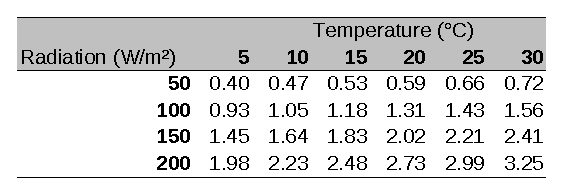
\includegraphics[width=0.9\columnwidth]{\figdir/makkink.eps}
\end{table}
